\documentclass{ctexart}
\usepackage{ctex}
\usepackage[nounderscore]{syntax}
\AtBeginDocument{\catcode`\_=8 }
\ctexset{section/format = {\Large\bfseries}}
\newenvironment{typewriterfont}{\ttfamily}{\par}
\usepackage{listings}
\usepackage{graphics}
\usepackage{geometry}
\geometry{left=3.0cm, right=3.0cm, top=2.0cm, bottom=2.0cm}

\title{Tigger文档说明}
\date{}
\author{}

\pagestyle{plain}

\begin{document}
\maketitle
\section{概述}
Tigger /\texttt{'}t\i g\textschwa (r)/ 是面向RISC-V的一种中间表示,用作寄存器分配的输出格式。

为了让同学们快速熟悉Tigger语法,Tigger遵循一贯的简洁易读风格,被设计得与Eeyore很像。

%Tigger在MiniC编译器中的地位,对应着MiniJava编译器中使用到的Kanga中间语言。

%Tigger这个名字与Kanga取自同一部动画。

\section{语法描述}
\subsection{寄存器}
Tigger共有28个可用的寄存器,这些寄存器的名称与RISC-V保持一致(相比RISC-V,删去了一些不需要编译器管理寄存器)。
\begin{itemize}
\item
\texttt{x0}:该寄存器恒等于0,不可更改

\item
\texttt{s0-s11}:没什么特殊之处,被调用者保存。

\item
\texttt{t0-t6}:没什么特殊之处,调用者保存。

\item
\texttt{a0-a7}:用来传递函数参数,调用者保存。其中a0-a1也被用作传递函数返回值,但因为MiniC中所有函数返回值都是int,所以实际上只有a0被用作传递返回值。
\end{itemize}
可以看出,最多只能通过寄存器传递8个参数。简单起见,限定所有函数参数个数不超过8个。

\subsection{表达式、标号、跳转语句}
\begin{itemize}
\item
所有的表达式计算都在寄存器上进行。

\item
所有在Eeyore中支持的运算符,在Tigger中都支持。

\item
注意!因为MiniC里只有int和int数组类型,所以形似数组赋值语句的赋值语句中括号内的数是4的倍数。

\item
注意!由于RISC-V某些规则的原因,Tigger中只有的\texttt{'+'}和\texttt{'<'}运算符允许作为\texttt{Reg = Reg OP2 <INTEGER>}语句中的\texttt{OP2}。

\item
标号与跳转语句和Eeyore中的语法相同,标号是全局的。
\end{itemize}
\subsection{函数}
\begin{itemize}
\item
函数定义语句形如\texttt{f\_xxx [2] [3]},第一个中括号内是参数个数,第二个是该函数需要用到的栈空间的大小(除以4之后)。

\item
函数结束语句和Eeyore中的一样,形如\texttt{end f\_xxx}。

\item
函数必须以返回语句返回。返回值通过寄存器传递。

\item
函数调用语句形如\texttt{call f\_xxx}。
\end{itemize}
\subsection{栈内存操作}
程序运行时,每个被调用的函数都会维护一个连续的栈空间,大小为函数定义语句中的第二个参数。

局部变量都可以在栈中找到,因此Tigger中不再有局部变量了。

\begin{itemize}
\item
\texttt{store Reg <INTEGER>}语句中,\texttt{<INTEGER>}是一个小于函数定义语句第二个系数的非负整数。该语句会把寄存器\texttt{<Reg>}的值存入当前函数栈空间第\texttt{<INTEGER>}个位置。

\item
\texttt{load <INTEGER> Reg}语句中,\texttt{<INTEGER>}是一个小于函数定义语句第二个系数的非负整数。该语句会把当前函数栈空间第\texttt{<INTEGER>}个整数存入寄存器\texttt{<Reg>}

\item
\texttt{loadaddr <INTEGER> Reg}语句中,\texttt{<INTEGER>}是一个小于函数定义语句第二个系数的非负整数。该语句会把当前函数栈空间第\texttt{<INTEGER>}个位置的内存地址存到寄存器\texttt{<Reg>}。
\end{itemize}

举个例子,假设某个时刻函数调用关系是\texttt{main[0][3] -> f[0][4]},正在执行函数\texttt{f},假设此时的栈如下图所示:

\begin{center}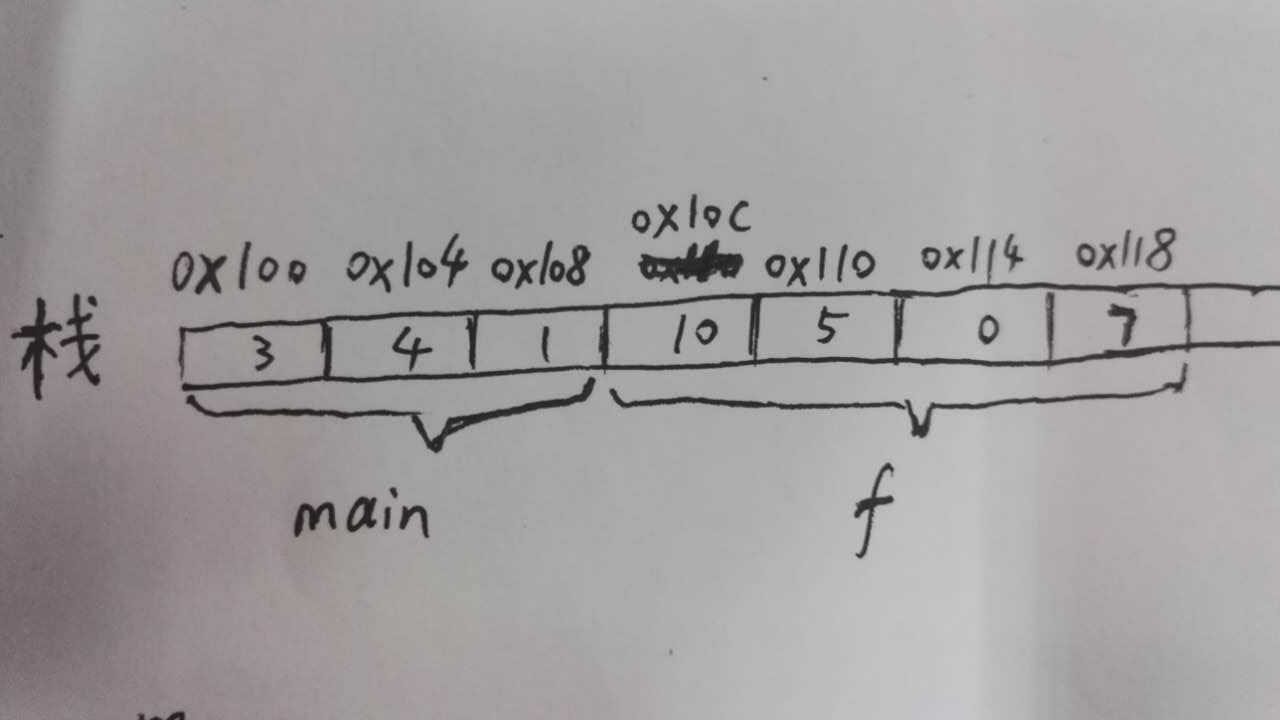
\includegraphics[width=6.4cm,height=3.6cm]{stack}\end{center}

此时语句\texttt{load 2 s0},会使\texttt{s0 = 5};语句\texttt{loadaddr 2 s0},会使\texttt{s0 = 0x110};语句\texttt{store s0 2}会把图中的\texttt{5}改成\texttt{s0}的值。

\subsection{全局变量}

\begin{itemize}
\item
全局变量名称以\texttt{v}开头,后接一个整数编号,编号从0开始,比如\texttt{v0,v1}。

\item
\texttt{<VARIABLE> = <INTEGER>}用来声明一个初始值为\texttt{<INTEGER>}的全局变量\texttt{<VARIABLE>},即\texttt{<VARIABLE>}这个名称表示的内存地址上4字节的内容为\texttt{<INTEGER>}。

\item
\texttt{<VARIABLE> = malloc <INTEGER>}用来声明数组,\texttt{<VARIABLE>}这个名称表示的内存地址之后的\texttt{<INTEGER>}字节的内容为一个数组。
注意!\texttt{<INTEGER>}是4的倍数。

%对全局变量的操作都通过寄存器完成,全局变量的\texttt{load}和\texttt{store}语句与之前介绍的稍有不同。

\item
\texttt{load <VARIABLE> Reg}表示把\texttt{<VARIABLE>}这个全局变量对应内存地址上4字节的内容加载到寄存器\texttt{Reg}。

\item
\texttt{loadaddr <VARIABLE> Reg}表示把\texttt{<VARIABLE>}这个全局变量对应内存地址加载到寄存器\texttt{Reg}。

\item
注意!由于RISC-V汇编的原因,没有\texttt{store Reg <VARIABLE>}语句。该语句可以通过\texttt{loadaddr}语句与数组访问语句结合来完成。
\end{itemize}

\subsection{注释}
Tigger允许单行注释,与C语言注释类似使用//,处理时自动忽略改行从//之后所有内容。

\subsection{系统库支持}
与MiniC和Eeyore中的输入输出函数原型相同。

四种输入输出函数都通过\texttt{a0}寄存器传递参数和返回值。

\newpage
\section{BNF}
\setlength{\grammarindent}{8em} % increase separation between LHS/RHS 
\begin{typewriterfont}
\begin{grammar}
<Goal>  ::= (FunctionDecl | GlobalVarDecl)*

<GlobalVarDecl> ::= <VARIABLE> '=' <INTEGER>
\alt <VARIABLE> '=' 'malloc' <INTEGER>

<FunctionDecl> ::= Function '['<INTEGER>']' '['<INTERGER>']' (Expression)* 'end' Function

<Expression>	::=	Variable '=' Reg OP2 Reg
\alt Reg '=' Reg OP2 <INTEGER>
\alt Reg '=' OP1 Reg
\alt Reg '=' Reg
\alt Reg '=' <INTEGER>
\alt Reg '[' <INTEGER> ']' = Reg
\alt Reg = Reg '[' <INTEGER> ']'
\alt 'if' Reg LogicalOP Reg 'goto' Label
\alt 'goto' Label
\alt Label ':'
\alt 'call' Function
\alt 'store' Reg <INTEGER>
%\alt 'store' Reg <VARIABLE>
\alt 'load' <INTEGER> Reg
\alt 'load' <VARIABLE> Reg
\alt 'loadaddr' <INTEGER> Reg
\alt 'loadaddr' <VARIABLE> Reg
\alt 'return'

<Reg> ::= 'x0'
| 's0'
| 's1'
| 's2'
| 's3'
| 's4'
| 's5'
| 's6'
| 's7'
| 's8'
| 's9'
| 's10'
| 's11'
| 'a0'
| 'a1'
| 'a2'
| 'a3'
| 'a4'
| 'a5'
| 'a6'
| 'a7'
| 't0'
| 't1'
| 't2'
| 't3'
| 't4'
| 't5'
| 't6'

<Label> ::= <LABEL>

<Function> ::= <FUNCTION>

\end{grammar}
\end{typewriterfont}

\newpage
\section{示例}
\begin{typewriterfont}
\begin{lstlisting}
f_fac [1] [3]
    a0 = a0 + -1
    if a0 <= x0 goto l1
    store a0 0
    call f_fac
    store a0 1
    store s0 2
    loadaddr 0 s0
    a0 = s0[0]
    a0 = a0 + -1
    call f_fac
    a1 = s0[4]
    load 2 s0
    a0 = a0 + a1
    goto l2
l1:
    a0 = 1
l2:
    return
end f_fac

f_main [0] [0]
    call f_getint
    call f_fac
    call f_putint
    a0 = 10
    call f_putchar
    a0 = 0
    return
end f_main
\end{lstlisting}
\end{typewriterfont}

\newpage
\section{Tigger模拟器使用方式}
\begin{typewriterfont}
\begin{lstlisting}
Usage ./Tigger [-d] <filename>

-d : enable debug mode

- e.g. ./Tigger -d test.in

出现"> "提示符表示进入debug模式,支持如下指令:

+ l
    - Print current line number
+ n
    - Run one step
+ pr <Reg>
    - e.g. pr a0, pr s0
    - Print register value
+ prx <Reg>
    - e.g. prx a0, prx s0
    - Print register value as hexadecimal
+ ps <stacknum>
    - e.g. ps 0, ps 1
    - Print the value of stack memory
+ psx <stacknum>
    - e.g. psx 0, psx 1
    - Print the value of stack memeory as hexadecimal
+ pg <variable>
    - e.g. pg v0, pg v1
    - Print the value of global variable
+ b <number>
    - e.g. b 10
    - Set a breakpoint at a certain line
+ d <number>
    - e.g. d 10
    - Delete the breakpoint at a certain line
+ c
    - Run until meet a breakpoint
+ q
    - Quit Tigger simulator
\end{lstlisting}
\end{typewriterfont}
\end{document}
